\chapter{Self-dual Higgs model}
\section{The EFT Lagrangian}
In hadron colliders, the dominant channel for the Higgs boson production is described by the interaction between two gluons through a top quark loop, known as gluon-gluon fusion. In order to compute QCD corrections, we can integrate out the heavy top quark describing the interaction between the Higgs and gluons through an effective coupling. We can construct the effective Lagrangian density considering the possible gauge invariant operators,
$$
	\mathcal{L}_{eff}=\frac{C}{2}\tr(G^{\mu\nu}G_{\mu\nu})H+D \tr(G^\mu_\nu G^\nu_\rho G^\rho_\mu) H + \dots
$$
From a dimensional analysis, we observe that the ratio $D/C$ is suppressed with the inverse of the top mass squared. Hence we consider only the first addend which produces the following rule,
\begin{equation}
	\feynmandiagram [small, horizontal=a to t1, baseline=(a.base)] {
a [particle=\(H\)] -- [scalar] t1 [crossed dot]-- [gluon, momentum=\(p_1\)] t2, t3 -- [gluon, rmomentum=\(p_2\)] t1 
};
=-iC \left(p_1\cdot p_2\right)\epsilon^*(p_1)\cdot \epsilon^*(p_2).	\label{effrule}
\end{equation}
We can fix the coefficient $C$ working with the Standard Model in the top mass limit. We explicitly show the computation at $\mathcal{O}(\alpha_s)$ computing the one-loop diagrams for $H\rightarrow gg$. 
\begin{equation}
 \begin{aligned}
i \mathcal{A}(H\rightarrow gg)= \feynmandiagram [small, horizontal=a to t1, baseline=(a.base)] {
a [particle=\(H\)] -- [scalar] t1 []-- [fermion] t2 -- [fermion] t3 -- [fermion] t1 [label={0:\(\hspace{0.4cm} t\)}], t2 -- [gluon, momentum'=\(p_2\)] p1 [particle=\(b\nu\)],
t3 -- [gluon, momentum=\(p_1\)] p2 [particle=\(a\mu\)]
};
+
 \feynmandiagram [small, horizontal=a to t1, baseline=(a.base)] {
a [particle=\(H\)] -- [scalar] t1 []-- [anti fermion] t2 -- [anti fermion] t3 -- [anti fermion] t1 [label={0:\(\hspace{0.4cm} t\)}], t2 -- [gluon, momentum'=\(p_2\)] p1 [particle=\(b\nu\)],
t3 -- [gluon, momentum=\(p_1\)] p2 [particle=\(a\mu\)]
};
\end{aligned}
\end{equation}
Using the Feynman rules of SM Lagrangian, we have
\begin{align*}
	i\mathcal{A}(H\rightarrow gg)=&\frac{i m_t}{v}g^2 \epsilon_\mu^*(p_1) \epsilon_\nu^*(p_2) \tr(T^a T^b) \int \frac{\dd^d q}{(2\pi)^d}\left\{-\tr\left[\gamma^\mu \frac{i}{\slashed q-m_t}\gamma^\nu \frac{i}{\slashed q+\slashed p_2 -m_t}\frac{i}{\slashed q-\slashed p_1-m_t}\right]\right.\\
		&\left.-\tr\left[\gamma^\nu \frac{i}{\slashed q-m_t}\gamma^\mu \frac{i}{\slashed q+\slashed p_1-m_t}\frac{i}{\slashed q-\slashed p_2-m_t}\right]\right\}
\end{align*}
where $v$ is the Higgs vev and $m_t$ the mass of top quark.\\
Introducing two Feynman parameters and using Ward identity $p^\mu_i \epsilon_\mu(p_i)=0$ to simplify the numerator, we obtain 
\begin{align*}
	i\mathcal{A}(H\rightarrow gg)=-\frac{2g^2 m_t}{v} \delta^{ab} \int_0^1 \dd x_1 \int_0^{1-x_1} \dd x_2 \int \frac{\dd^d q}{(2\pi)^d} \frac{N_{\mu\nu}}{(q^2-m_t^2+x_1x_2 m_H^2)^3} \epsilon_\mu^*(p_1) \epsilon_\nu^*(p_2)
\end{align*}
with the numerator
$$
	N_{\mu\nu}=4 m_t \left[m_t^2+\left(x_1x_2-\frac{1}{2}\right)m_H^2+\frac{4-d}{d}q^2\right]
$$
where $m_H$ is the Higgs mass. We have to carefully set the limit $d\rightarrow 4$ indeed $N_{\mu\nu}$ presents an infinitesimal quantity which produces a finite contribution when we multiply it with the divergent tensor integral evaluated in dimensional regularisation.\\
Introducing the strong coupling $\alpha_s=\tfrac{g^2}{4\pi}$, the amplitude becomes 
\begin{align*}
i\mathcal{A}(H\rightarrow gg)=-\frac{i\alpha_s}{8\pi v}\delta^{ab} \epsilon_\mu^*(p_1) \epsilon_\nu^*(p_2) \int_0^1 \dd x_1 \int_0^{1-x_1} \dd x_2 \frac{4x_1 x_2 -1}{1-x_1x_2 \left(\frac{m_H}{m_t}\right)^2}m_H^2.
\end{align*}
In conclusion we take the limit top mass limit, hence in the Standard Model framework the color ordered stripped matrix element for the process $H\rightarrow gg$ is
\begin{align}
	iA(H\rightarrow gg)=-i \frac{\alpha_s}{6\pi v} \epsilon_\mu^*(p_1) \epsilon_\nu^*(p_2).
\end{align}
This result can be compared with (\ref{effrule}) in order to deduce the value of the effective coupling,
$$
	C=\frac{\alpha_s}{6\pi v}+\mathcal{O}(\alpha_s^2).
$$
The constant $C$ is currently known at $\mathcal{O}(\alpha_s^4)$ \cite{Chetyrkin:1997iv}.
\subsection{Self-dual Higgs $\phi$}
The MHV structure of Higgs+gluon amplitudes is best described by dividing the effective interaction into two terms. Firstly, we introduce a pseudo-scalar field $A$ and consider the Lagrangian density,
\begin{align*}
	\mathcal{L}^{\text{int}}_{H,A}=\frac{C}{2}\left[H\, \text{tr}\left( G_{\mu\nu}G^{\mu\nu}\right)+iA\,\text{tr}\left( G_{\mu\nu}*G^{\mu\nu}\right)\right].
\end{align*}
Introducing the complex field $\phi=H+iA$, we observe the following re-organisation,
\begin{align}
\mathcal{L}^{\text{int}}_{H,A}=C\left[\phi\, \text{tr}\left( G_{SD\mu\nu}G_{SD}^{\mu\nu}\right)+\phi^\dagger\, \text{tr}\left( G_{ASD\mu\nu}G_{ASD}^{\mu\nu}\right)\right]	\label{lagrangian}
\end{align}
where we introduced the self-dual and anti self-dual gluon field strength,
\begin{align*}
	G_{SD}^{\mu\nu}\equiv\frac{1}{2}(G^{\mu\nu}+*G^{\mu\nu}),\hspace{0.5cm}G_{ASD}^{\mu\nu}\equiv\frac{1}{2}(G^{\mu\nu}-*G^{\mu\nu}), \hspace{0.5cm} *G^{\mu\nu}\equiv \frac{i}{2}\epsilon^{\mu\nu\rho\sigma} G_{\rho\sigma}.
\end{align*}
Due to its interaction term, the $\phi$ field is called \text{self-dual Higgs}. The key idea is that due to the self-duality the amplitudes with these complex fields, $\phi$ and $\phi^\dagger$, show a simpler structure. Hence, Higgs amplitudes will be obtained as a sum of two contributions at any loop order in our perturbative expansion,
$$
	\mathcal{A}^{\ell L}(H; 1^{h_1}2^{h_2}\dots n^{h_n}) =\mathcal{A}^{\ell L}(\phi; 1^{h_1}2^{h_2}\dots n^{h_n}) +\mathcal{A}^{\ell L}(\phi^\dagger; 1^{h_1}2^{h_2}\dots n^{h_n}). 
$$
The amplitudes with $\phi$ and $\phi^\dagger$ are related by parity,
$$
	\mathcal{A}^{\ell L}(\phi; 1^{h_1}2^{h_2}\dots n^{h_n})=\left[\mathcal{A}^{\ell L}(\phi^\dagger; 1^{-h_1}2^{-h_2}\dots n^{-h_n})\right]_{\langle ij \rangle \leftrightarrow [ji]}.
$$
This re-organisation of the degrees of freedoms can be argued by embedding the interaction into an $\mathcal{N}=1$ supersymmetric effective Lagrangian \cite{Dixon_2004}.
\section{$\phi$+gluon tree amplitudes}
The self-dual Higgs is colorless, then the color decomposition for the $\phi$+gluon amplitudes is equivalent to the QCD case. We will explicitly extract the effective constant $C$ in order to simplify the expression of partial amplitudes. Then, for tree-level amplitudes which describe the interaction between $\phi$ and $n$ gluons, we use the trace based decomposition,
\begin{align*}
	\mathcal{A}^{tree}(\phi; 1^\pm, 2^\pm, \dots, n^\pm)=g^{n-2} C \sum_{\sigma\in S_n /\mathbb{Z}_n} \tr(T^{a_{\sigma_1}}T^{a_{\sigma_2}}\dots T^{a_{\sigma_n}}) A^{tree}(\phi;\sigma(1),\sigma(2),\dots, \sigma(3)).
\end{align*}
\subsection{Explicit computation of $\phi+2g$}
We start to study the interaction between two (off-shell) gluons and the self-dual Higgs,
\begin{align}
	\feynmandiagram [small, horizontal=a to t1, baseline=(a.base)] {
a [particle=\(\phi\)] -- [scalar] t1 -- [gluon, momentum=\(k_1\)] t2 [particle=\(a\mu\)], t3 [particle=\(b\nu\)]-- [gluon, rmomentum=\(k_2\)] t1 
};
=\eta_{\mu\nu} k_1\cdot k_2 -k_{1\nu} k_{2\mu}+i\epsilon_{\mu\nu\rho\sigma}k_1^\rho k_2^\sigma=: V_{\mu\nu}(k_1,k_2)	\label{vertex:phigg}
\end{align}
Let us consider the helicity amplitudes. In the all-plus sector, the interaction is described by
\begin{align*}
	V(\phi;1^+,2^+):=\epsilon_+^\mu(k_1) V_{\mu\nu}(k_1,k_2) \epsilon_+^\nu (k_2) = -(k_1 \cdot \epsilon_+(k_2))(k_2 \cdot \epsilon_+(k_1))\left[1-\frac{i\epsilon_{\mu\nu\rho\sigma} k_1^\rho k_2^\sigma \epsilon_+^\mu (k_1) \epsilon_+^\nu (k_2)}{(k_1 \cdot \epsilon_+(k_2))(k_2 \cdot \epsilon_+(k_1))}\right],
\end{align*}
where we used the property $\epsilon_+ (k_1) \cdot \epsilon_+ (k_2)=0$.\\
The term proportional to the Levi-Civita tensor,
\begin{align*}
	T_{++}:=&-\frac{i\epsilon_{\mu\nu\rho\sigma} k_1^\rho k_2^\sigma \epsilon_+^\mu (k_1) \epsilon_+^\nu (k_2)}{(k_1 \cdot \epsilon_+(k_2))(k_2 \cdot \epsilon_+(k_1))}=-\frac{1}{4}\frac{\tr(\gamma_5 \slashed 	\epsilon_+(k_1)\slashed \epsilon_+(k_2) \slashed k_1 \slashed k_2)}{(k_1\cdot \epsilon_+(k_2))(k_1\cdot \epsilon_+(k_2))},
\end{align*}
can be simplified writing $\epsilon_+$ in terms of spinor products (\ref{solepsilon}) and using the Fierz rearrangement. The result is $T_{++}=-1$ which yields to $V(\phi;1^+,2^+)=0$.\\The only difference in the computation of $V(\phi;1^-,2^-)$ is a sign in the contribution proportional to $\epsilon_{\mu\nu\rho\sigma}$, then the two non-trivial addends sum together producing a non-vanishing vertex
\begin{align}
	V(\phi;1^-,2^-)=-2(k_1\cdot \epsilon_-(k_2))(k_2 \cdot \epsilon_-(k_1)).	\label{phi2g}
\end{align}
By writing the polarization in terms of spinors, we obtain the non-vanishing amplitude with two gluons,
\begin{align}
	A^{tree}(\phi;1^-,2^-)=-\langle 12 \rangle^2.	\label{phi2g}
\end{align}
In the case of two gluons with opposite helicity, we can observe that the amplitude with a $\phi$ field vanishes for angle-momentum conservation. Alternatively, one can directly prove it by showing that
\begin{align*}
	V(\phi;1^+,2^-):=&\ \epsilon_+^\mu(k_1) V_{\mu\nu}(k_1,k_2) \epsilon_-^\nu (k_2)\\
	\propto&\  \langle n\gamma^\mu 1] \langle 2 \gamma_\mu n] \tfrac{1}{2} \langle 12 \rangle [21]-\langle n 2 1]\langle 21n]=0
\end{align*}
where we introduced the generic direction $n$ to describe the polarization vectors. Using Fierz identity, one immediately sees that $V(\phi;1^+,2^-)$ vanishes.
\subsection{Vanishing helicity amplitudes}
Using off-shell currents and Berends-Giele recursion relations, we can show that \cite{Dixon_2004}
\begin{align*}
	A^{tree}(\phi;1^\pm,2^+,3^+,\dots, n^+)=0.		\label{vanamp}
\end{align*}
In order to construct it recursively, we have to attach gluon currents with the possible interaction vertices with $\phi$. From the Lagrangian (\ref{lagrangian}),  we can extract the Feynman rules, then we have to consider vertices involving the $\phi$ field and $2$, $3$ or $4$ gluons. We will call these vertices $V_{\mu\nu}, V_{\mu\nu\rho}, V_{\mu\nu\rho\sigma}$ and Berends-Giele currents will be attached to them.
\begin{align*}
	A(\phi;1^\pm,2^+,\dots,n^+)&=\sum_{k=1}^{n-1}  \left[V_{\mu\nu} J^\mu(1^\pm,2^+,\dots k^+) J^\nu((k+1)^+,\dots n^+)\right]+\sum_{k=1}^{n-2} \sum_{l=k+1}^{n-1} \left[V_{\mu\nu\rho} J^\mu(1^\pm,2^+,\dots k^+) \right.\\
	&\left.J^\nu((k+1)^+,\dots l^+) J^\rho((l+1)^+,\dots n^+)\right] +\sum_{k=1}^{n-3} \sum_{l=k+1}^{n-2} \sum_{m=l+1}^{n-1} \left[V_{\mu\nu\rho\sigma} J^\mu(1^\pm,2^+,\dots k^+) \right.\\ &\left.J^\nu((k+1)^+,\dots l^+) J^\rho((l+1)^+,\dots m^+) J^\sigma((m+1)^+,\dots, n^+)\right]
\end{align*}
Using the explicit expression of the currents \cite{Dixon:1996wi,Berends:1987me}, one can prove the following relations,
\begin{align*}
	&J_+ \cdot J_+= J_+ \cdot J_-=0,\\
	&\epsilon_{\mu\nu\rho\sigma} J^\mu_- J^\nu_+ J^\rho_+=0,
\end{align*}
where
$$
	J^\mu_{+}\equiv J^\mu(1^+,2^+,\dots, a^+), \hspace{0.5cm} J^\mu_-\equiv J^\mu(1^-,2^+,\dots, b^+).
$$
Hence, the addends vanish if they contain the Levi-Civita tensor contracted to at least three-currents or the metric attached to two currents. We remain only with the contribution from the $\phi+2g$ vertex. Similarly to the case $\phi+2g$, using Fierz identity we can show that
$$
	V_{\mu\nu} J^\mu(1^\pm, 2^+, \dots, k^+)J^\nu((k+1)^+,\dots, n^+)=0.
$$
Then, the $\phi$+gluon amplitudes vanish at tree-level in the all-plus sector or if we consider a single gluon with a negative helicity.
\subsection{MHV amplitudes} \label{MHVsection}
The first set of non trivial amplitudes requires two gluons with negative helicity. The structure is identical to the Parke-Taylor formula (\ref{PT}),
\begin{align}
	A^{tree}(\phi;1^+,\dots, i^-,\dots, j^-, \dots, n^+)=\frac{\langle ij \rangle^4}{\langle 12 \rangle \langle 2 3\rangle \dots \langle (n-1)n\rangle\langle n 1 \rangle}.	\label{MHVphi}
\end{align}
The only difference with the pure QCD case is the presence of an additional colorless field which changes the momentum conservation law,
\begin{align*}
	\sum_{i=1}^n p_i^\mu=-p_\phi^\mu\not =0.
\end{align*}
We can prove (\ref{MHVphi}) using BCFW relations \cite{Berger:2006sh}. For simplicity, using the cyclic property of the partial amplitude, we can focus on $A^{tree}(\phi;1^-,2^+,\dots, j^-, \dots, n^+)$.
We can consider the shift of momenta $p_1$ and $p_n$ so that
\begin{align}
	\begin{cases}
		\hat p_1(z)=p_1-z\eta,\\
		\hat p_n(z)=p_n+z\eta,
	\end{cases}\,
	\begin{cases}
		| \hat 1 ] = | 1] - z | n ],\\
		| \hat n \rangle = | n \rangle + z | 1 \rangle.
	\end{cases}
	\label{shift}
\end{align}

Before applying the recursion relations, we have to verify the hypothesis about the large shift behavior of the amplitude. Firstly, a triple gluon vertex is proportional to $z$ in the large limit because it contains a momentum, while quartic vertices goes like constant due to the absence of momentum factors. In contrast to the pure QCD case, in this theory we have an effective vertex (\ref{vertex:phigg}) which contains terms with two momenta. The $z^2$-contributions of $V_{\mu\nu}(\hat p_1, \hat p_n)$ which come from $\eta_{\mu\nu}$ and $\epsilon_{\mu\nu\rho\sigma}$-terms clearly vanish, while the non-trivial one is the behavior of the second term. However, in the large shift limit $\hat p_1$ and $\hat p_n$ become proportional to each other since their sum $-p_\phi$ is order $z^0$. Then we can use the current conservation $$\hat p_n \cdot \hat J_1 \sim \hat p_1 \cdot \hat J_1=0$$ which holds also for complex momenta. This shows that in the effective theory the new vertices contain only $z$-contributions in the large shift limit, like the triple gluon interaction.\\
Then the most divergent graph is obtained by considering only cubic vertices, say $r$. We have to include $(r-1)$ propagators and we also attach the polarization vectors $\epsilon^-(\hat p_1)$ and $\epsilon^+(\hat p_n)$ which goes like $1/z$. In conclusion, we obtain the following behavior for the amplitude,
$$
	A(z)\sim \frac{z^{r+1}}{z^r} z^{-2}=\frac{1}{z}, \text{ for }z\rightarrow \infty.
$$
Then, there is no contributions from the residue at infinity, so BCFW relation should work. Firstly, we study the case of three gluons in which there is only the following contribution, 
\begin{align*}
	A(\phi;1^-,2^-,3^+)=A^{tree}(\phi;\hat 1^-, (\hat P_{2,3})^-)\frac{1}{P_{2,3}^2} A^{tree}(2^-,\hat 3^+, -(\hat P_{2,3})^+)
\end{align*}
This amplitude can be computed using (\ref{phi2g}) in order to check the MHV formula in the case of three gluons.\\
At higher multiplicity, we have again only one non-vanishing contribution. Indeed, on the right-hand side of the BCFW relation, we have to consider a sub-amplitude with only one gluon with negative helicity. For this reason, the only non-vanishing contribution comes from the triple gluon interaction.
\begin{align*}
	&A^{tree}(\phi;1^-,2^+,\dots, j^-,\dots, n^+)=\left[\begin{aligned}
	\feynmandiagram [small, horizontal=b to a] {
	a  -- [gluon, rmomentum=\(\hspace{0.2cm}\hat P_{n-1,n}^{+}\)] b [blob, label={180:\(\bullet\,\)}, label={90:\(\bullet\hspace{0.3cm}\)}] -- [gluon] f1 [particle=\((n-2)^+\)], b -- [gluon] f2 [particle=\(j-\)],
	b -- [gluon] pt3 [particle=\(\hat 1^-\)],
	b -- [scalar] pt [particle=\(\phi\)],
	}	;
	\end{aligned}\right] \frac{1}{P^2_{n-1,n}}
	\left[\begin{aligned}
	\feynmandiagram [small, layered layout, horizontal=a to b] {
	a  -- [gluon, rmomentum=\(-\hat P_{n-1,k}^{-}\)] b [blob] -- [gluon] f1 [particle=\(\hat n^+\)], b -- [gluon] f2 [particle=\((n-1)^+\)],
	}	;
	\end{aligned}\right]\\
	&\hspace{1cm}=A^{tree}(\phi; 1^-,2^+,\dots,j^-,(n-2)^+, (\hat P_{n-1,n})^+)\frac{1}{ P_{n-1,n}^2} A^{tree}((n-1)^+,\hat n^+,(-\hat P_{n-1,n})^-)\\
	&\hspace{1cm}=\frac{\langle 1j \rangle^4}{\langle \hat 12 \rangle \dots \langle (n-2)\hat P_{n-1,n} \rangle \langle \hat P_{n-1,n} \hat 1 \rangle}\frac{1}{s_{n-1,n}}\frac{[(n-1) \hat n]^3}{[\hat n (-\hat P_{n-1,n})][(-\hat P_{n-1,n}) (n-1)]}\\
	&\hspace{1cm}=\frac{\langle 1j \rangle ^4 [(n-1)n]^2}{\langle 12\rangle \dots \langle (n-3)(n-2)\rangle \langle (n-1) n \rangle \langle (n-2) P_{n-1,n} n] \langle 1 P_{n-1,n} (n-1)]}=\frac{\langle 1j \rangle^4}{\langle 12 \rangle \dots \langle (n-1)n \rangle \langle n1 \rangle}
\end{align*}
Hence, we reviewed the proof of the correctness for (\ref{MHVphi}) by induction using BCFW recursion relation.
\subsection{Anti-MHV amplitudes}
An other infinite set of amplitudes is the so-called anti-MHV tower characterised by all-minus gluons. The interaction between $\phi$ and gluons with negative helicity is related by parity with $\phi^\dagger$+gluon amplitudes in the all-plus configuration.\\
These amplitudes can be computed using off-shell Berends-Giele recursion relations. The difference with the $\phi+$gluon case is that the three-point vertex $V(\phi^\dagger;1^+,2^+)$ does not vanish due to an additional term in front of the Levi-Civita term. We can show that \cite{Dixon_2004}
\begin{align}
	A^{tree}(\phi^\dagger; 1^+,2^+,\dots, n^+)=\frac{s_\phi^2}{\langle 12 \rangle \langle 23 \rangle \dots \langle n1 \rangle},	\label{resnow}
\end{align}
where $s_\phi$ is the Higgs mass squared. Since the $\phi$ amplitude with positive gluons vanishes, the result (\ref{resnow}) represents also the all-plus Higgs amplitude.\\
Then, we can extract the $\phi$ amplitude in the all-minus sector,
\begin{align*}
	A^{tree}(\phi;1^-,2^-,\dots,n^-)=(-1)^n\frac{s_\phi^2}{[12][23]\dots [n1]}.
\end{align*}
We discussed only particular sets of tree-level amplitudes we will use later. However, it is possible to deduce amplitudes with different helicity configurations using recursion relations \cite{Dixon_2004}.

%%%%-----Non presente
\iffalse
We can organize the non-vanishing tree-level helicity amplitudes using the following plot.
\begin{figure}[H]
\begin{center}
  	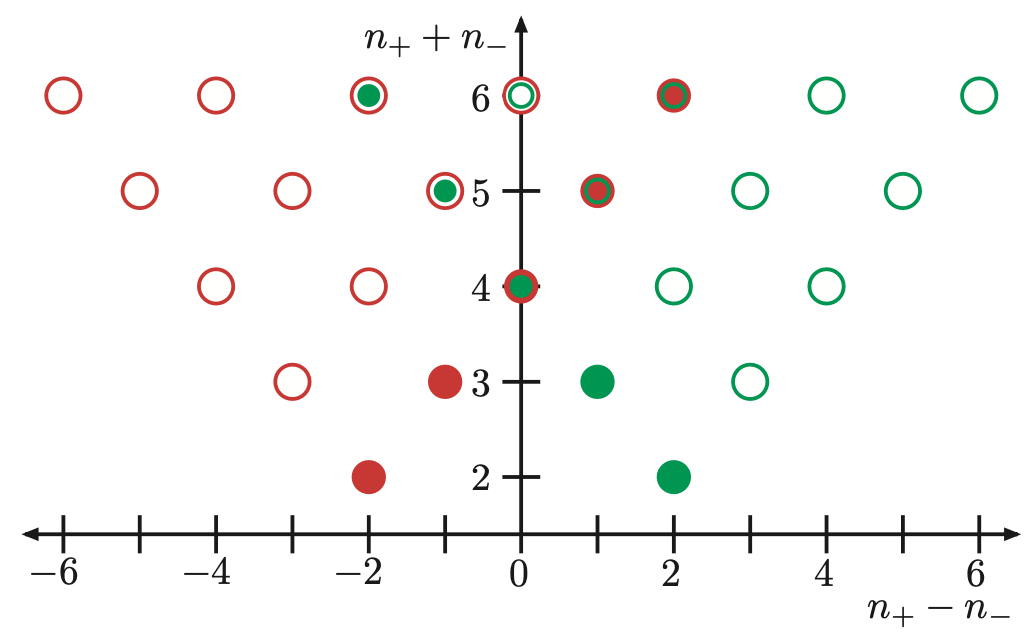
\includegraphics[width=0.4\textwidth]{MHVplot}
	\caption{Plot of number of gluons in terms of the difference in positive and negative helicity.}
\end{center}
\end{figure}
\fi
\iffalse
\begin{equation}
\begin{aligned}	
\tikzfeynmanset{ myblob/.style={ shape=circle, typeset=$nL$,
draw=black, } }
    \feynmandiagram [large, horizontal=b to c, baseline=(d.base)] {
      c -- [gluon] b [myblob, label={90:\(\text{\hspace{0.2cm}}\bullet\)}, label={70:\(\bullet\)}, label={30:\(\bullet\)}] -- [gluon] a,
      b -- [scalar] d [particle=\(H\)],
      f -- [gluon] b -- [white] e,
      g -- [gluon] b,
    };=
    \feynmandiagram [large, horizontal=b to c,  baseline=(d.base)] {
      c -- [gluon] b [myblob, label={90:\(\text{\hspace{0.2cm}}\bullet\)}, label={70:\(\bullet\)}, label={30:\(\bullet\)}] -- [gluon] a,
      b -- [scalar] d [particle=\(\phi\)],
      f -- [gluon] b -- [white] e,
      g -- [gluon] b,
    };+
    \feynmandiagram [large, horizontal=b to c,  baseline=(d.base)] {
      c -- [gluon] b [myblob, label={90:\(\text{\hspace{0.2cm}}\bullet\)}, label={70:\(\bullet\)}, label={30:\(\bullet\)}] -- [gluon] a,
      b -- [scalar] d [particle=\(\phi^\dagger\)],
      f -- [gluon] b -- [white] e,
      g -- [gluon] b,
    };
\end{aligned}
 \end{equation}
\begin{eqnarray*}
	\tikzfeynmanset{ my2blob/.style={ shape=circle, typeset=tree,
draw=black, } }
\begin{tikzpicture}[baseline=(current bounding box.center)]
  \begin{feynman}
    \diagram [horizontal=b to c] {
           b [my2blob] -- [gluon] a [particle=\(1^+\)], 
           b -- [gluon] w1 [particle=\(4^+\)],
      b  -- [scalar] d1 [particle=\(\phi\)],
      b -- [gluon] w2 [particle=\(2^+\)],
      b -- [gluon] d [ particle=\(3^+\)],
    };
  \end{feynman}
\end{tikzpicture}\scalebox{1.6}{$\stackrel{\text{on-shell}}{=}\,0$}
\end{eqnarray*}
\fi
%%%----Fine sezione
\section{One-loop all-plus $\phi$ amplitude}
We use the standard trace-based color decomposition with double traces at one-loop,
\begin{align}
	\mathcal{A}^{1L}(\phi;1,2,\dots,n)=g^nC\,c_\Gamma \sum_{c=1}^{\lfloor n/2 \rfloor+1} \sum_\sigma Gr_{n;c} A^{1L}_{n,c}\left(\phi;\sigma(1,2,\dots,n)\right).	\label{phidec1l}
\end{align}
where $\lfloor x \rfloor$ is the largest integer less than or equal to $x$ and $c_\Gamma$ is the standard loop factor. In the large $N_C$ limit the leading structure is
$$
	Gr_{n;1}(1)=N_C \Tr\left(T^{a_1}T^{a_2}\dots T^{a_n}\right),
$$
and we focus on the kinematical contribution attached to this color factor, $A^{1L}_{n,1}(\phi;1,\dots,n)$, which we will denote as $A^{1L}(\phi;1\dots, n)$.\\
The simplest one-loop partial amplitude describe the interaction between the $\phi$ field and all-plus gluons. The cut-constructible part is absent because any double cut requires the product of two trees and at least one of them vanishes due to (\ref{vanamp}). Then, this amplitude is purely rational. It was derived in \cite{Berger:2006sh} using recursion relations after an explicit computation in the case of two gluons,
\begin{align}
	A^{1L}(\phi;1^+,2^+,\dots n^+)=\frac{-2s_\phi^2}{\langle 12 \rangle \langle 23 \rangle \dots \langle n1 \rangle} =-2 A^{tree}(\phi^\dagger;1^+,2^+,\dots,n^+).	\label{1Lphi}
\end{align}
As already done for QCD amplitudes, we can separate the amplitude into contributions with different type of particles in the loop,
\begin{align}
	A^{1L}(\phi;1^+,2^+,\dots,n^+)=A^{1L[g]}+\frac{n_f}{N_C} A^{1L[f]}+\frac{n_s}{N_C} A^{1L[s]}=A^{1L[g-s]}+\left(\frac{d_s-2}{2}-\frac{n_f}{N_C}+\frac{n_s}{N_C}\right) A^{1L[s]}.
\end{align}
$A^{1L[g]}$ comes from gluon loops and the fermion contribution $A^{1L[f]}$ is opposite to the scalar one $A^{1L[s]}$. $A^{1L[g-s]}$ describes the difference between gluon and scalar effects.\\
Let us start considering the amplitude at the lowest multiplicity. The terms from fermion and scalar loops vanish and we have to compute only the gluon contribution,
\begin{align*}
	A^{1L}(\phi;1^+,2^+)=A^{1L[g]}=\left[
	\begin{aligned}
	\begin{tikzpicture}[scale=0.65,baseline=(current bounding box.center)]
 	 \begin{feynman}
    		\diagram [small, vertical=d to c] {
      			d2 [particle=\(\phi\)] -- [scalar] b -- [gluon] c
        			-- [gluon] d  -- [gluon] b,
      			d4 -- [gluon] c,
      			d -- [gluon] s ,
   		 };
  	\end{feynman}
	\end{tikzpicture}
	\end{aligned}+
	\begin{aligned}
	\begin{tikzpicture}[scale=0.65,baseline=(current bounding box.center)]
 	 \begin{feynman}
    		\diagram [small, horizontal=d2 to b] {
      			d2 [particle=\(\phi\)] -- [scalar] b -- [gluon, half right] c,
			c  -- [gluon, half right] b,
      			d4 -- [gluon] c,
      			c -- [gluon] s ,
   		 };
  	\end{feynman}
	\end{tikzpicture}
	\end{aligned}\right]=\frac{-2s_\phi^2}{\langle 12 \rangle \langle 21 \rangle}.
\end{align*}
The previous amplitude is the starting point of our recursion relation at one-loop level \cite{Bern_2005}. The computation is similar to the proof of MHV formula in section [\ref{MHVsection}]. We use the shift (\ref{shift}) and we observe that there is only a single contribution,
\begin{align*}
	A^{1L}(\phi;1^+,\dots,n^+)=A^{1L}(\phi;\hat 1^+,2^+,\dots, (n-1)^+, \hat P_{n-1,n}^+)\frac{1}{s_{n-1,n}} A^{tree}((n-1)^+,\hat n^+,(-\hat P_{n-1,n})^-),
\end{align*}
which shows the correctness of (\ref{1Lphi}).\\

Another rational set of one-loop $\phi$+gluon amplitudes is characterised by only one gluon with negative helicity \cite{Berger:2006sh}. The other $\phi$ amplitudes show discontinuities. For example we can see branch cuts studying the all-minus amplitude which was computed in \cite{Badger_2006}. 

\section{$\phi$ amplitudes with gluons and a quark-antiquark pair}
Another interesting set of amplitudes involves also a quark-antiquark pair. We will study pure QCD corrections to $\phi$+gluon amplitudes without considering quarks effects, but it is interesting to notice some properties if the theory has a couple of fermions.

These two partons do not interact directly with the self-dual Higgs. We have to consider at least an external gluon, indeed in the case of massless quarks $\mathcal{A}(\phi, 1_q, 2_{\bar q})$ vanishes due to angular momentum conservation.\\
At tree-level the $\phi$ amplitude with two quarks and all-plus gluons is zero,
\begin{align*}
	\mathcal{A}^{tree}(\phi,1_q^-, 2^+, \dots, j_{\bar q}^+,(j+1)^+, \dots, n^+)=0,
\end{align*}
and it is rational at one-loop \cite{Berger:2006sh}.